\clearpage
\setcounter{page}{1}
\maketitlesupplementary
\section{数据集}  
表 \ref{tab:MPReID} 展示了 MPReID 的组成,而表 \ref{tab:HMReID}、表 \ref{tab:GibsonReID} 和表 \ref{tab:ReplicaReID} 分别展示了 HMReID、GibsonReID 和 ReplicaReID 的组成。表 \ref{tab:Statistics} 报告了每个房间 ReID 数据集中语义上不同房间的数量。

\begin{table}[ht]
\centering
\vspace{-3pt}
\resizebox{\columnwidth}{!}{
\begin{tabular}{c|c|c|c|c|c}
\toprule
\textbf{Scene} & \textbf{Rooms} & \textbf{Images} & \textbf{Scene} & \textbf{Rooms} & \textbf{Images} \\
\midrule
8WUmhLawc2A & 8 & 1232 & EDJbREhghzL & 7 & 1078 \\
RPmz2sHmrrY & 5 & 770 & S9hNv5qa7GM & 9 & 1423 \\
ULsKaCPVFJR & 5 & 780 & VzqfbhrpDEA & 7 & 1078 \\
WYY7iVyf5p8 & 4 & 616 & X7HyMhZNoso & 7 & 1078 \\
YFuZgdQ5vWj & 7 & 1078 & i5noydFURQK & 7 & 1078 \\
jh4fc5c5qoQ & 5 & 770 & mJXqzFtmKg4 & 9 & 1386 \\
qoiz87JEwZ2 & 8 & 1232 & wc2JMjhGNzB & 11 & 1708 \\
yqstnuAEVhm & 6 & 924 & \textbf{Total} & \textbf{105} & \textbf{16231} \\
\bottomrule
\end{tabular}
}
\vspace{-1em}
\caption{MPReID 的组成。}
\label{tab:MPReID}
\end{table}

\vspace{-1em}

\begin{table}[ht]
\centering
\resizebox{\columnwidth}{!}{
\begin{tabular}{c|c|c|c|c|c}
\toprule
\textbf{Scene} & \textbf{Rooms} & \textbf{Images} & \textbf{Scene} & \textbf{Rooms} & \textbf{Images} \\
\midrule
7dmR22gwQpH & 6 & 924 & ACZZiU6BXLz & 5 & 682 \\
CETmJJqkhcK & 5 & 813 & CFVBbU9Rsyb & 5 & 770 \\
Coer9RdivP7 & 3 & 462 & DZsJKHoqEYg & 5 & 793 \\
EQSguCqe5Rk & 5 & 819 & Fgtk7tL8R9Y & 5 & 822 \\
GLAQ4DNUx5U & 7 & 1156 & GcfUJ79xCZc & 5 & 572 \\
NcK5aACg44h & 5 & 754 & P8L1328HrLi & 5 & 819 \\
VSxVP19Cdyw & 5 & 769 & b3CuYvwpzZv & 5 & 690 \\
ixTj1aTMup2 & 5 & 757 & ochRmQAHtkF & 5 & 641 \\
qWb4MVxqCW7 & 6 & 879 & rrjjmoZhZCo & 5 & 704 \\
w7QyjJ3H9Bp & 5 & 692 & zR6kPe1PsyS & 5 & 803 \\
zepmXAdrpjR & 3 & 460 & \textbf{Total} & \textbf{105} & \textbf{15781} \\
\bottomrule
\end{tabular}
}
\vspace{-1em}
\caption{HMReID 的组成。}
\label{tab:HMReID}
\end{table}

\vspace{-1em}

\begin{table}[ht]
\centering
\resizebox{\columnwidth}{!}{
\begin{tabular}{c|c|c|c|c|c}
\toprule
\textbf{Scene} & \textbf{Rooms} & \textbf{Images} & \textbf{Scene} & \textbf{Rooms} & \textbf{Images} \\
\midrule
Ackermanville & 1 & 154 & Angiola & 1 & 154 \\
Avonia & 2 & 308 & Beach & 3 & 462 \\
Branford & 1 & 154 & Brevort & 1 & 154 \\
Cason & 2 & 262 & Cooperstown & 2 & 308 \\
Corder & 2 & 308 & Creede & 4 & 526 \\
Elmira & 2 & 308 & Eudora & 2 & 308 \\
Fredericksburg & 2 & 308 & Greigsville & 1 & 154 \\
Idanha & 1 & 154 & Laytonsville & 3 & 462 \\
Lynxville & 2 & 308 & Mahtomedi & 2 & 257 \\
Mayesville & 2 & 308 & Northgate & 1 & 154 \\
Ogilvie & 2 & 308 & Ophir & 3 & 462 \\
Pablo & 1 & 154 & Sumas & 2 & 308 \\
- & - & - & \textbf{Total} & \textbf{45} & \textbf{6743} \\
\bottomrule
\end{tabular}
}
\vspace{-1em}
\caption{GibsonReID的组成。}
\label{tab:GibsonReID}
\end{table}

\vspace{-1em}

\begin{table}[ht]
\centering
\resizebox{\columnwidth}{!}{
\begin{tabular}{c|c|c|c|c|c}
\toprule
\textbf{Scene} & \textbf{Rooms} & \textbf{Images} & \textbf{Scene} & \textbf{Rooms} & \textbf{Images} \\
\midrule
apartment\_0 & 3 & 462 & apartment\_1 & 1 & 154 \\
apartment\_2 & 4 & 616 & frl\_apartment\_0 & 3 & 426 \\
hotel\_0 & 1 & 154 & office\_0 & 1 & 154 \\
office\_2 & 1 & 140 & office\_3 & 1 & 140 \\
office\_4 & 1 & 154 & room\_0 & 1 & 154 \\
room\_1 & 1 & 154 & room\_2 & 1 & 154 \\
- & - & - & \textbf{Total} & \textbf{19} & \textbf{2862} \\
\bottomrule
\end{tabular}
}
\vspace{-1em}
\caption{ReplicaReID 的组成。}
\label{tab:ReplicaReID}
\end{table}

\begin{table}[h]
\centering
\resizebox{\columnwidth}{!}{
\begin{tabular}{c|c|c|c|c|c|c|c|c|c|c|c|c|c|c}
\hline
 & bathroom & kitchen & living & office & bedroom & theater & dining & wardrobe & gym & laundry & garage & storage & nursery & supermarket \\
\hline
MPReID & 13 & 13 & 20 & 3 & 41 & 4 & 4 & 2 & 2 & 2 & 1 & 0 & 0 & 0 \\
\hline
HMReID & 10 & 18 & 29 & 8 & 31 & 0 & 3 & 1 & 0 & 1 & 0 & 2 & 2 & 0 \\
\hline
GibsonReID & 2 & 10 & 11 & 3 & 12 & 0 & 1 & 0 & 3 & 1 & 0 & 1 & 0 & 1 \\
\hline
ReplicaReID & 0 & 2 & 6 & 6 & 3 & 0 & 2 & 0 & 0 & 0 & 0 & 0 & 0 & 0 \\
\hline
\end{tabular}
}
\caption{四个新构建的房间ReID数据集中语义不同房间的统计数据。}
\label{tab:Statistics}
\end{table}
\section{实验细节}

\subsection{整体性能比较}
\label{sec:appendix_overall}

\paragraph{基准配置} 对于CVNet,我们使用ResNet50作为骨干网络,并将降维维度设置为2048。对于DINOv2,我们使用DINOv2-Base检查点。对于Patch-NetVLAD,我们加载在Pittsburgh数据集上优化的预训练权重,应用WPCA来将特征嵌入维度降低到4096,设置RANSAC作为匹配器,使用0.45、0.15和0.4的补丁权重,配置补丁大小为2、5和8,步幅为1。对于AnyLoc,我们采用AnyLoc-VLAD-DINOv2,使用DINOv2 ViT-G/14架构,将描述符层设置为31,使用VLAD并设置32个聚类,指定域为\mbox{室内}。

\paragraph{基准适配} 对于CVNet和Patch-NetVLAD,我们通过选择前5个候选项进行全局检索,然后进行重新排序。对于CVNet,选择具有最高CVNet-Rerank图像相似度得分的候选项作为最终结果;而对于Patch-NetVLAD,则选择在成对局部匹配阶段具有最高RANSAC得分的参考项。对于DINOv2和AnyLoc,从查询和参考图像中提取全局特征,并计算余弦相似度。选择具有最高余弦相似度得分的参考图像作为最终匹配项。

\paragraph{AirRoom配置} 对于全局特征提取器,我们使用AnyLoc-VLAD-DINOv2,采用DINOv2 ViT-G/14架构,将描述符层设置为31,应用VLAD并设置32个聚类,指定域为室内。对于实例分割,我们采用Semantic-SAM,并使用来自SA-1B的预训练权重和SwinL骨干网络。物体特征提取器使用在ImageNet数据集上预训练的ResNet50模型实现。对于细粒度检索,我们使用LightGlue,并将最大关键点数设置为2048。
\subsection{按组性能比较}

\paragraph{基线配置} 对于ResNet50主干网络组,ResNet50和CVNet的配置遵循\sref{sec:appendix_overall}中详细介绍的设置。对于NetVLAD主干网络组,我们使用NetVLAD与VGG-16作为特征提取器,配置为64个聚类和512维特征。对于Patch-NetVLAD,特征维度分别设置为4096、512和128,其余设置与\sref{sec:appendix_overall}一致。

\paragraph{基线适配} 对于ResNet50主干网络组,ResNet50从查询图像和参考图像中提取全局特征,并使用余弦相似度选择得分最高的参考图像作为最终匹配。CVNet的适配过程详见\sref{sec:appendix_overall}。对于NetVLAD主干网络组,NetVLAD从查询图像和参考局部特征中聚合全局描述符,并选择余弦相似度得分最高的参考图像作为最终结果。Patch-NetVLAD的适配过程同样遵循\sref{sec:appendix_overall}。

\paragraph{AirRoom配置} 对于ResNet50主干网络组,ResNet50作为全局特征提取器,配置与\sref{sec:appendix_overall}一致。对于NetVLAD主干网络组,NetVLAD作为全局特征提取器,配置遵循本节中“基线配置”段落中的设置。两组中其余模块的配置也与\sref{sec:appendix_overall}一致。
\subsection{管道灵活性评估}

\subsubsection{全局特征提取器}

\paragraph{基准配置} 对于ViT,我们使用Base变体,补丁大小为16,输入图像大小为224×224,并加载来自ImageNet的预训练权重。对于DINO,我们采用DINO预训练的Vision Transformer Small (ViT-S/16)变体。DINOv2的配置遵循\sref{sec:appendix_overall}。对于AnyLoc,VLAD聚类设置为16和8,其他所有配置与\sref{sec:appendix_overall}一致。

\paragraph{基准适配} 所有基准用于从查询图像和参考图像中提取特征,计算余弦相似度,以识别具有最高相似度得分的参考房间。

\paragraph{AirRoom配置} 为了与主干基准进行比较,主干被用作全局特征提取器。主干配置遵循本节“基准配置”段落中概述的内容,而AirRoom中其余模块的配置与\sref{sec:appendix_overall}一致。
\subsubsection{实例分割}

\paragraph{AirRoom 配置} DINOv2 被用作全局特征提取器。对于 Mask R-CNN,我们使用带有 ResNet50 主干和 FPN 的 Mask R-CNN,并加载在 COCO 上训练的预训练权重。对于 Semantic-SAM,我们使用带有从 SA-1B 预训练的权重和 SwinL 主干的 Semantic-SAM。其余模块的配置与 \sref{sec:appendix_overall} 一致。
\section{大规模评估}
由于四个房间ReID数据集采用了一致的格式,我们在它们的联合数据集上评估我们的方法,这样可以为每种房间类型提供更多的样本,并评估在数据扩展时所提出方法的可行性。为此,我们通过将所有四个数据集合并,构建了一个大规模数据集UnionReID。表 \ref{tab:Union} 展示了AirRoom与四种基线方法的性能比较,表明在大规模条件下,AirRoom仍然优于它们。

\begin{table}[h]
\centering
\resizebox{\columnwidth}{!}{
\begin{tabular}{l|cccc}
\toprule
\multirow{2}{*}{\textbf{Methods}} & \multicolumn{4}{c}{\textbf{UnionReID}} \\
 & Accuracy & Precision & Recall & F1 \\
\midrule
CVNet & 14.10 & 27.53 & 14.10 & 16.19 \\
DINOv2 & 53.01 & 59.44 & 53.02 & 53.50 \\
Patch-NetVLAD & 61.15 & 67.53 & 61.04 & 62.31 \\
AnyLoc & 88.28 & 89.62 & 88.22 & 88.32 \\
\rowcolor{Lavender} AirRoom & \textbf{91.87} & \textbf{92.55} & \textbf{91.76} & \textbf{91.76} \\
\bottomrule
\end{tabular}
}
\caption{在 UnionReID 上与基线模型的对比,用于评估 AirRoom 在数据扩展下的性能。}
\label{tab:Union}
\end{table}
\section{室内定位数据集评估}
严格来说,房间重识别(Room ReID)是一项新任务,尚无先前建立的数据集,并且与室内定位任务有本质区别。为了填补这一空白,我们引入了四个新数据集。然而,在审查现有的室内定位数据集后,我们识别出两个勉强可用的数据集:InLoc \cite{taira2018inlocindoorvisuallocalization} 和 Structured3D \cite{Structured3D}。InLoc \cite{taira2018inlocindoorvisuallocalization} 采用基于区域的划分,而非基于房间的划分,其中一些图像仅捕捉走廊和角落。Structured3D \cite{Structured3D} 包含数万个房间实例,但每个房间的视角少于六个。这些局限性减少了这两个数据集的适用性,尽管它们仍然在某种程度上可用。然而,在这些数据集上评估我们的方法仍能进一步加强其验证。

表 \ref{tab:Indoor} 展示了在这两个室内定位数据集上的比较结果,结果表明,AirRoom 始终优于其他方法。此外,由于 InLoc 代表了更为现实的实际环境,结果进一步证明了 AirRoom 在实际环境中的鲁棒性。

\begin{table}[h]
\vspace{-7pt}
\centering
\resizebox{\columnwidth}{!}{
\begin{tabular}{l|cccc|cccc}
\toprule
\multirow{2}{*}{\textbf{Methods}} & \multicolumn{4}{c|}{\textbf{InLoc}} & \multicolumn{4}{c}{\textbf{Structured3D}} \\
 & Acc & Prec & Rec & F1 & Acc & Prec & Rec & F1 \\
\midrule
CVNet & 8.41 & 12.49 & 8.41 & 8.99 & 12.60 & 21.39 & 12.60 & 14.22 \\
DINOv2 & 11.13 & 19.93 & 11.13 & 11.85 & 53.00 & 63.60 & 53.00 & 54.04 \\
Patch-NetVLAD & 12.78 & 19.59 & 12.78 & 13.73 & 56.30 & 67.67 & 56.30 & 57.71 \\
AnyLoc & 15.78 & 26.11 & 15.78 & 17.04 & 73.40 & 79.75 & 73.40 & 73.90 \\
\rowcolor{Lavender} AirRoom & \textbf{16.80} & \textbf{26.36} & \textbf{16.80} & \textbf{18.05} & \textbf{76.20} & \textbf{82.88} & \textbf{76.20} & \textbf{76.70} \\
\bottomrule
\end{tabular}
}
\caption{在现有数据集上与基线模型的对比,以进一步验证我们的方法。}
\label{tab:Indoor}
\end{table}
\section{运行时分析}

在本节中,我们评估了每个模块的运行时,并将我们的管道的总运行时与几种最先进的方法进行比较,以评估我们方法的效率。

\begin{table}[ht]
\centering
\resizebox{\columnwidth}{!}{
\begin{tabular}{l|cccccc}
\toprule
\multirow{2}{*}{\textbf{Modules}} & \multicolumn{6}{c}{\textbf{Runtime (ms)}} \\
 & t=0 & t=0.1 & t=0.2 & t=0.3 & t=0.4 & t=0.5 \\
\midrule
Global Feature Extractor & 48.8 & 44.1 & 43.2 & 44.0 & 43.0 & 43.8 \\
Global Retrieval & 0.1 & 0.1 & 0.1 & 0.1 & 0.1 & 0.1 \\
Instance Segmentation & 38.7 & 38.1 & 38.2 & 38.1 & 38.0 & 38.0 \\
Receptive Field Expander & 6.9 & 2.9 & 1.7 & 1.3 & 0.9 & 0.7 \\
Object Feature Extractor & 113.7 & 71.3 & 47.0 & 33.3 & 29.0 & 22.8 \\
Object-Aware Scoring & 2.9 & 2.2 & 1.7 & 1.5 & 1.4 & 1.2 \\
Fine-Grained Retrieval & 87.4 & 86.3 & 86.1 & 86.1 & 85.8 & 86.2 \\
\midrule
\textbf{Total} & \textbf{299.9} & \textbf{246.5} & \textbf{219.4} & \textbf{205.7} & \textbf{199.5} & \textbf{194.2} \\
\bottomrule
\end{tabular}
}
\caption{Mask R-CNN \& ResNet 运行时间。}
\label{tab:module_runtime_mr}
\end{table}

\begin{table}[ht]
\centering
\resizebox{\columnwidth}{!}{
\begin{tabular}{l|cccccc}
\toprule
\multirow{2}{*}{\textbf{Modules}} & \multicolumn{6}{c}{\textbf{Runtime (ms)}} \\
 & t=0 & t=0.1 & t=0.2 & t=0.3 & t=0.4 & t=0.5 \\
\midrule
Global Feature Extractor & 65.0 & 58.6 & 52.7 & 50.2 & 48.6 & 47.9 \\
Global Retrieval & 0.1 & 0.1 & 0.1 & 0.1 & 0.1 & 0.1 \\
Instance Segmentation & 38.4 & 38.8 & 38.6 & 38.7 & 38.6 & 38.5 \\
Receptive Field Expander & 7.9 & 3.2 & 1.8 & 1.3 & 1.0 & 0.7 \\
Object Feature Extractor & 146.9 & 86.9 & 55.6 & 40.9 & 32.3 & 26.3 \\
Object-Aware Scoring & 2.9 & 2.2 & 1.7 & 1.5 & 1.4 & 1.2 \\
Fine-Grained Retrieval & 87.0 & 87.4 & 87.0 & 87.1 & 87.5 & 87.3 \\
\midrule
\textbf{Total} & \textbf{349.5} & \textbf{278.6} & \textbf{238.8} & \textbf{221.1} & \textbf{210.9} & \textbf{203.4} \\
\bottomrule
\end{tabular}
}
\caption{Mask R-CNN \& DINOv2 运行时间。}
\label{tab:module_runtime_md}
\end{table}

\begin{table}[ht]
\centering
\resizebox{\columnwidth}{!}{
\begin{tabular}{l|cccccc}
\toprule
\multirow{2}{*}{\textbf{Methods}} & \multicolumn{6}{c}{\textbf{Accuracy (\%)}} \\
 & t=0 & t=0.1 & t=0.2 & t=0.3 & t=0.4 & t=0.5 \\
\midrule
AirRoom-MaskRCNN-ResNet & 92.70 & 92.68 & 92.58 & 92.59 & 92.22 & 92.15 \\
AirRoom-MaskRCNN-DINOv2 & 87.67 & 87.62 & 87.10 & 87.20 & 87.24 & 87.09 \\
\bottomrule
\end{tabular}
}
\caption{Mask R-CNN \& ResNet / DINOv2 准确率。}
\label{tab:module_accuracy}
\end{table}

\begin{figure}[ht]
    \centering
    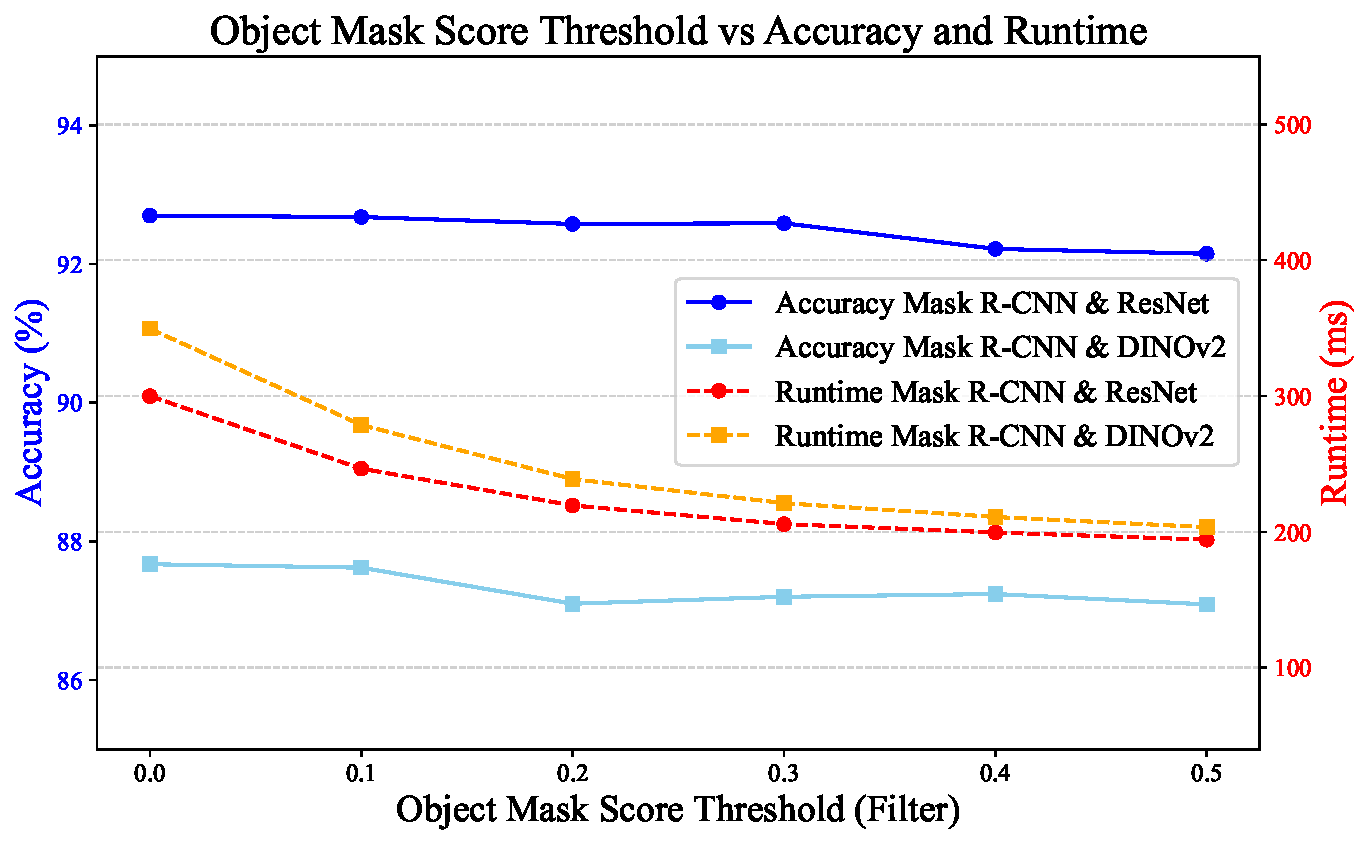
\includegraphics[width=\columnwidth]{runtime.pdf}
    \caption{随着目标掩码评分阈值的提高,AirRoom 的性能略有下降;然而,效率却显著提升。}
    \label{fig:runtime}
\end{figure}

\begin{table}[ht]
\centering
\begin{tabular}{l|cc}
\toprule
\multirow{2}{*}{\textbf{Modules}} & \multicolumn{2}{c}{\textbf{Runtime (ms)}} \\
 & ResNet & DINOv2 \\
\midrule
Global Feature Extractor & 42.5 & 56.2 \\
Global Retrieval & 0.1 & 0.1 \\
Instance Segmentation & 352.6 & 343.2 \\
Receptive Field Expander & 0.7 & 0.6 \\
Object Feature Extractor & 51.1 & 66.6 \\
Object-Aware Scoring & 2.2 & 2.1 \\
Fine-Grained Retrieval & 87.8 & 87.4 \\
\midrule
\textbf{Total} & \textbf{538.5} & \textbf{557.6} \\
\bottomrule
\end{tabular}
\caption{Semantic-SAM \& ResNet / DINOv2 运行时间。}
\label{tab:module_runtime_ssam}
\end{table}

\begin{table}[ht]
\centering
\begin{tabular}{l|c|c}
\toprule
\textbf{Methods} & \textbf{Runtime (ms)} & \textbf{Accuracy (\%)}\\
\midrule
CVNet & 111.3 & 11.71 \\
DINOv2 & \textbf{16.7} & 53.91 \\
Patch-NetVLAD & 100.5 & 64.86 \\
AnyLoc & 45.5 & 89.69 \\
\rowcolor{Lavender} AirRoom & 194.2 & \textbf{92.15} \\
\bottomrule
\end{tabular}
\caption{与当前最先进方法的运行时间比较。}
\label{tab:runtime_comparison}
\end{table}

当使用 Mask R-CNN 进行实例分割时,\tref{tab:module_runtime_mr} 证明了当使用 ResNet 时,提高目标掩模分数阈值会显著减少对象特征提取器的运行时。这是由于需要处理的对象和补丁数量减少所致。使用 DINOv2 作为对象特征提取器时,\tref{tab:module_runtime_md} 中也观察到类似的趋势。此外,\tref{tab:module_accuracy} 显示,AirRoom 的性能在对象掩模分数阈值升高时保持基本不变,无论选择哪种对象特征提取器。这一观察在 \fref{fig:runtime} 中得到了进一步说明。然而,当使用 Semantic-SAM 进行实例分割时,由于 Semantic-SAM 显著较慢的性能,AirRoom 面临效率上的挑战,具体内容见 \tref{tab:module_runtime_ssam}。

\tref{tab:runtime_comparison} 比较了不同方法的运行时。AirRoom 比 CVNet 多需要 80ms,但实现了超过 80\% 的性能提升。与 Patch-NetVLAD 相比,AirRoom 的运行时大约是其两倍,性能提升超过 30\%。虽然 DINOv2 完成任务需要 10–20ms,AirRoom 增加了 170ms 并提升了超过 40\% 的性能。相较于 AnyLoc,AirRoom 增加了约 150ms 的运行时,但捕获了额外的 20\% 性能潜力。这些结果表明,尽管在有限的改进空间内,AirRoom 仍能提供显著的性能提升,突显了其在运行时上的有效性。

目前,AirRoom 为细粒度检索分配了约 90ms,使用 LightGlue 进行特征匹配。探索更轻量和更快速的替代方案可以进一步提高效率。在如实时导航等实际应用中,房间重识别时间在 50–200ms 之间通常是可接受的,精度是主要考虑因素。虽然 AirRoom 比一些基线稍慢,但它实现了显著的精度提升,有效地平衡了运行时和性能。这使得 AirRoom 非常适合实际场景,能够满足现实世界的运行时要求,同时保持高可靠性和精确度。
